\section{Results}
\begin{figure}[h]
    \centering
    \includegraphics[width=14cm]{img/camvolution_running.jpg}
    \caption[The implemented system running]{
        An image of a flower is sent from a laptop using HDMI.
        The image is convolved by the Camvolution board and sent to a screen.
    }
    \label{fig:systemRunning}
\end{figure}

In this section, the results of the groups work is presented.
All the individual components worked when tested independently and a demonstration bit file assembled with a slimmed down version of the convolution processor successfully outputted processed data, bypassing both EBI and SRAM completely.
This is presented in more detail below.

\subsection{Convolution in Software with Chisel}
Before the Camvolution system was implemented in hardware,
the convolution engine was tested and found to correctly perform convolution in Chisel software tests.

\begin{figure}[h]
    \centering
    \begin{subfigure}{7cm}
        \centering
        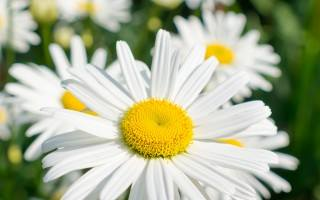
\includegraphics[width=6.5cm]{img/daisysmallorig.jpg}
        \caption{Original image}
    \end{subfigure}
    \begin{subfigure}{7cm}
        \centering
        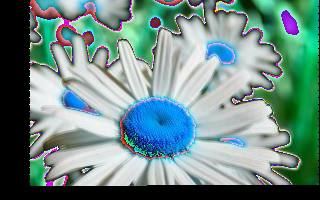
\includegraphics[width=6.5cm]{img/daisysmall.jpg}
        \caption{After convolution}
    \end{subfigure}
    \caption[Software simulated convolution]{
        Convolution performed in software simulation with Chisel
    }
    \label{fig:soft_sim}
\end{figure}

\subsection{HDMI Timing}
When sending HDMI data directly from input to output without delaying the signal, the control signal from the input HDMI signals can be used as output control signals.
This results in perfect synchronisation with the top left corner of the input being displayed in the top left corner on the screen.

When processing the data, the data is delayed and arrives too late compared to the control signals. This results in a image shifted slightly to the right as can be seen in Figure \ref{fig:SyncDelay}.

\begin{figure}
    \centering
    \includegraphics[width=14cm]{img/red_green_test.jpg}
    \caption[The delayed data stream]{
        The delayed data stream shows up as a shifted image.
        The laptop displays the original input signal and the screen behind displays the output.
        A 3x3 matrix of ones is used as kernel.
    }
    \label{fig:SyncDelay}
\end{figure}

\subsection{Slimmed Down Processor}
The processor implemented in the final design does not do true convolution as the Chisel design gave no output on the display when used to configure the FPGA.
Due to time constraints, the bug was never found, but a simpler version of the processor, without the input and output handlers, was found to be working.

As the input and output handlers take care of reordering the input data before performing the convolution, the data is fed through the processor in an incorrect order.
In practice this results in the convolution being applied to 9 consecutive pixels instead of a 3x3 square.
This can also be seen in Figure \ref{fig:SyncDelay} as a yellow regions between the red and blue squares in the output image.
Notice that this does not happen in the vertical direction as the image is sent through the processor in a row-major order.

Visible in Figure \ref{fig:Overflow} are vertical lines not present in the input.
The lines are caused by the processor being designed to run some rows twice since a sweep of 9 input rows only produces 7 output rows.
Figure \ref{fig:soft_sim} a shows how the output looks when input and output is handled correctly in software.

Also missing from the slimmed down version of the processor is the possibility of setting convolution kernel and operators on run-time.
Instead, several versions of the bit file was stored to the SD card for testing.
Buttons on the MCU were set up to load the next bit file when pushed.

\subsection{Overflow}
Another artefact in the design is especially visible when gradients are displayed, as demonstrated in Figure \ref{fig:Overflow}.
As the data width is the same through the entire processor, the values generated when adding several pixels together exceeds the maximum value that can be represented by the data format used.

These values wrap around and is offset by the maximum value, causing an otherwise wide spectrum to be split into several spectrum with the same dynamic range as the original.

\begin{figure}
    \centering
    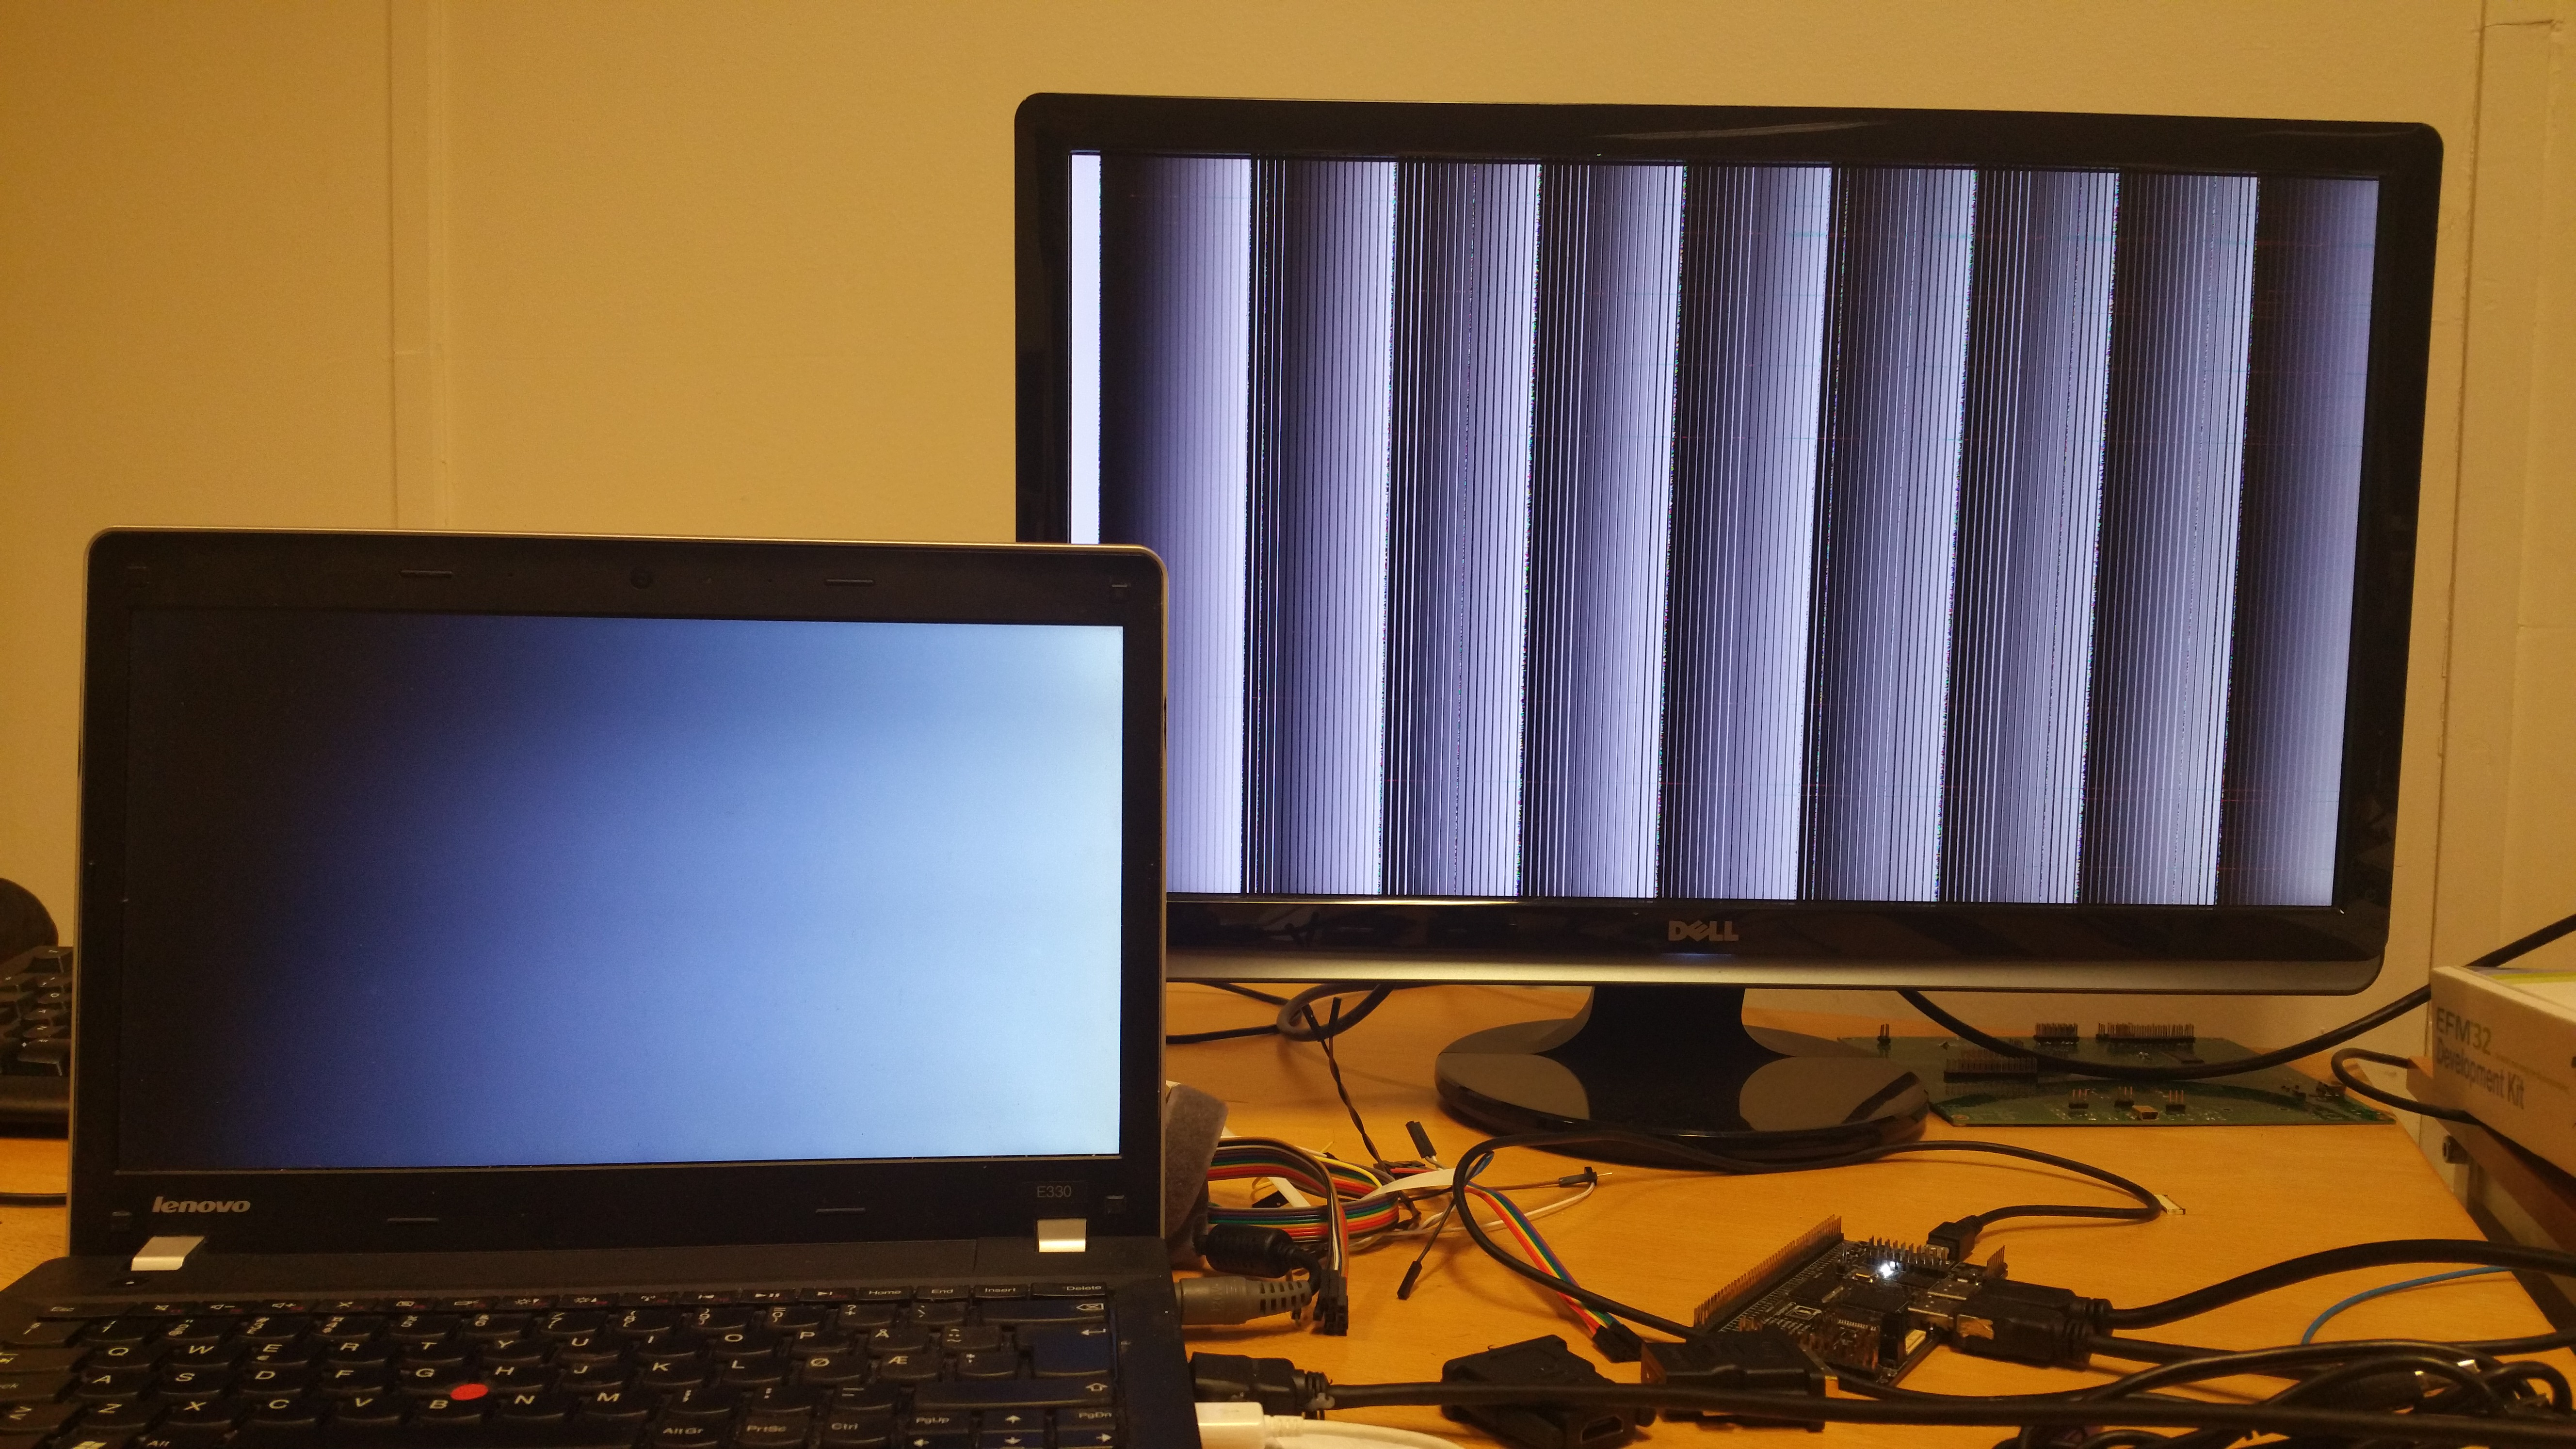
\includegraphics[width=14cm]{img/gradient_test}
    \caption[Gradient Output]{
        The laptop displays the input image, the display behind displays the output.
        The original gradient is turned into several shorter periods due to overflow when accumulating the final values.
        A 3x3 matrix of ones is used as kernel.
    }
    \label{fig:Overflow}

\end{figure}

\subsection{HDMI Channel Path}
After the first test of HDMI output from HDMI input, the HDMI input pins for R and B were swapped in the FPGA constraints to produce a picture with correct colour values.
The underlying problem were the HDMI output channels being swapped in the constraints. 
This led to the HDMI channel path for R and B through the FPGA to be remapped twice as shown in Figure \ref{fig:hdmiChannelPath}.
The image will have the correct colours at the output, but since VSYNC and HSYNC signals are only sent over channel B, information used to synchronise the image is lost.
By swapping the corresponding output channels instead of the input channel, a picture with correct colours as well as VSYNC and HSYNC signals appeared on the display.

\begin{figure}[h!]
    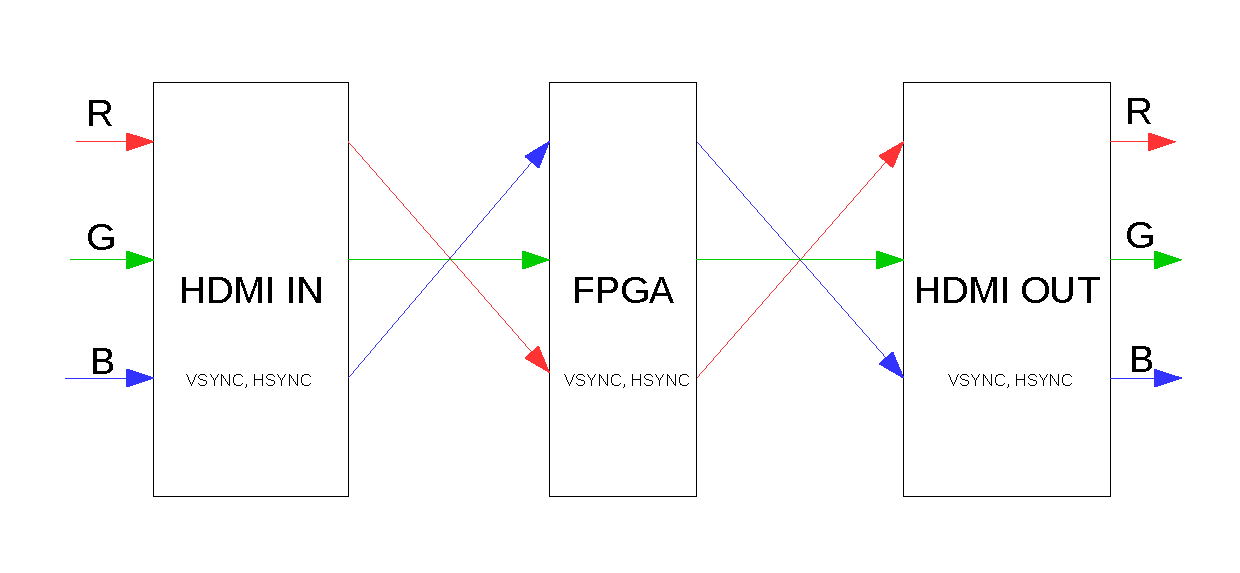
\includegraphics[width=\linewidth]{img/hdmi_channel_path.pdf}
    \caption[HDMI channels being swapped in the FPGA constraints]{
        HDMI channels being swapped in the FPGA constraints, VSYNC and HSYNC is lost
    }
    \label{fig:hdmiChannelPath}
\end{figure}

\subsection{Scalability}
As stated in Section \ref{sec:processor}, the processor has several parameters, some of which are hard coded into the final design.
These parameters can be adjusted, but many are limited by the available hardware.

In the final implementation the kernel values, map operands and reduce operands were hard coded for each configuration file.
This does not scale well with multiple configurations, as a small change in any of these parameters would need its own configuration file.
The time it takes for the MCU to program the FPGA with a new configuration file is about \unit[3]{seconds}.

In the final implementation HDMI frame synchronisation signals are being passed from input to output without going through the processor.
This means thatthe resolution of the image output is dependent on the input.

The size of the kernel matrices are hard coded both in the final design and in the final implementation.
To use larger kernel matrix sizes, it is possible to generate new configuration files capable of processing these.

According to the reports produced by Xilinx ISE during building of the FPGA bit file, the design for 3x3 convolution utilised around 16\% of the total number of available slices.

Since each component in the core of the processor only relies on its neighbours the processor can tackle large kernels without sacrificing clock speed.
The limiting factor is fast memory since data has to be buffered in order to be delivered as sweep slices.
The modularity of the processor allows it to be duplicated, letting as many cores as feasible work in parallel since convolution has no data dependency issues.
On our available hardware block ram and input bandwidth was the limiting factor, however on different hardware we believe instantiating many cores with different parameters should be a simple task.

\subsection{Video Throughput}
The highest correctly working resolution was found to be 1366x768.
This worked in real time with no perceivable delay. 1600x900 was also tried and found to be working, but resulted in an unexpected image with more artefacts. Finally, 1920x1200 was tried, but no sensible output was detected by the display.

